\documentclass[12pt, twoside]{article}
\usepackage[letterpaper, margin=1in, headsep=0.5in]{geometry}
\usepackage[english]{babel}
\usepackage[utf8]{inputenc}
\usepackage{amsmath}
\usepackage{amsfonts}
\usepackage{amssymb}
\usepackage{tikz}
\usetikzlibrary{quotes, angles}
\usepackage{graphicx}
%\usepackage{pgfplots}
%\pgfplotsset{width=10cm,compat=1.9}
%\usepgfplotslibrary{statistics}
%\usepackage{pgfplotstable}
%\usepackage{tkz-fct}
%\usepackage{venndiagram}
\usepackage{multicol}


\usepackage{fancyhdr}
\pagestyle{fancy}
\fancyhf{}
\fancyhead[LE]{\thepage}
\fancyhead[RO]{\thepage \\ Name: \hspace{4cm} \,\\}
\fancyhead[LO]{BECA / Dr. Huson / Geometry 10th Grade\\* Unit 6: Distance \& slope\\* 11 December 2019}

\renewcommand{\headrulewidth}{0pt}

\begin{document}
\subsubsection*{6.11b Do Now: Transformations and review\\[0.25cm]
(complete 12 stars per group)}
  \begin{enumerate}

  \begin{multicols}{2}
    [\item A dilation with $k=3$ centered at the origin maps $\triangle DEF$ onto $\triangle LMN$.] \vspace{0.5cm}
      The following is given:\\*[0.5cm]
      $DE=7.5$ \\
      $m\angle E = 43^\circ$ \\
      $m\angle F = 108^\circ$ \\
      $m\angle M = 5x + 8^\circ$ \\
      Fill in the blanks: \hfill (1 star each. 4 total)
      \begin{enumerate}
        \item $D \rightarrow$ \rule{2cm}{0.15mm}
        \item $LM =$ \rule{2cm}{0.15mm}
        \item $m\angle M =$ \rule{2cm}{0.15mm}
        \item Solve for $x$
      \end{enumerate}
    \end{multicols}  \vspace{3cm}

  \item What translation maps $\triangle ABC$ onto $\triangle DEF$, shown below? Fully specify the transformation.  \hfill (2 stars)\\[0.25cm]
    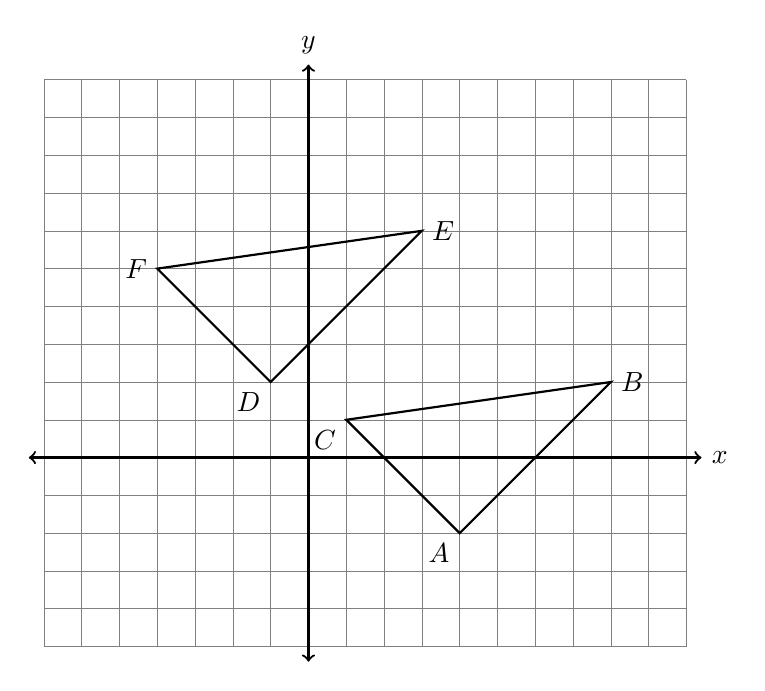
\begin{tikzpicture}[scale=.48]
      \draw [help lines] (-7,-5) grid (10,10);
      \draw [thick, <->] (-7.4,0) -- (10.4,0) node [right] {$x$};
      \draw [thick, <->] (0,-5.4)--(0,10.4) node [above] {$y$};  
      \draw [thick]
      (4,-2) node[below left] {$A$}--
      (8,2) node[right] {$B$}--
      (1,1) node[below left] {$C$}--cycle;  
      \draw [thick]
      (-1,2) node[below left] {$D$}--
      (3,6) node[right] {$E$}--
      (-4,5) node[left] {$F$}--cycle; 
    \end{tikzpicture}


  \item A translation maps $X(1,6) \rightarrow X'(-2,9)$. What is the image of $Y(10,-2)$ under the same translation? \hfill (2 stars)

\newpage
  \item Given isosceles $\triangle ABC$ with $\overline{AC} \cong \overline{AB}$, $m\angle A = x$, $m\angle B = 57$, and $m\angle C=y$. Mark and label the triangle, then find $x$ and $y$. \hfill (\emph{the diagram is not to scale})(2 stars)
  \begin{flushright}
  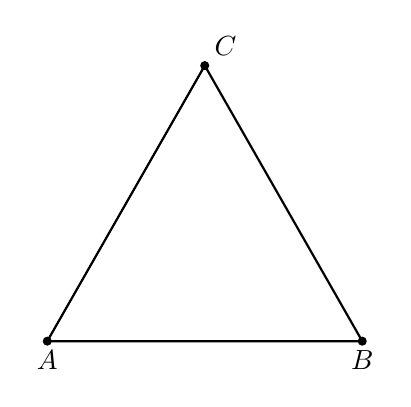
\begin{tikzpicture}[scale=1]
    \draw [thick](0,0)--(4,0)--(2,3.5)--(0,0);
    \draw [fill] (0,0) circle [radius=0.05] node[below]{$A$};
    \draw [fill] (4,0) circle [radius=0.05] node[below]{$B$};
    \draw [fill] (2,3.5) circle [radius=0.05] node[above right]{$C$};
  \end{tikzpicture}
  \end{flushright}

  \item Given isosceles $\triangle RSU$ with $\overline{UR} \cong \overline{RS}$. If $m\angle UST=130$ find $m\angle U$. (Mark and label the diagram) \hfill (\emph{the diagram is not to scale})(2 stars)
  \begin{flushright}
  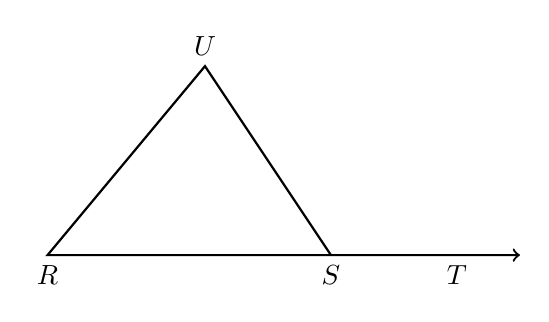
\begin{tikzpicture}[scale=0.8]
    %\draw [->, thick] (0,0)--(5,5);
    \draw [<-, thick] (8,0)--
      (7,0) node[below]{$T$}--
      (0.5,0) node[below]{$R$}--
      (3,3) node[above]{$U$}--
      (5,0) node[below]{$S$};
  \end{tikzpicture}
  \end{flushright} \vspace{1cm}

    \item Given parallel lines $\overleftrightarrow{AB} \parallel \overleftrightarrow{CDE}$ with $\overline{AC} \cong \overline{AD}$. If $m\angle BAD=70$ find $m\angle ACD$. (completely mark and label the diagram) \hfill (3 stars)
    \begin{flushright}
    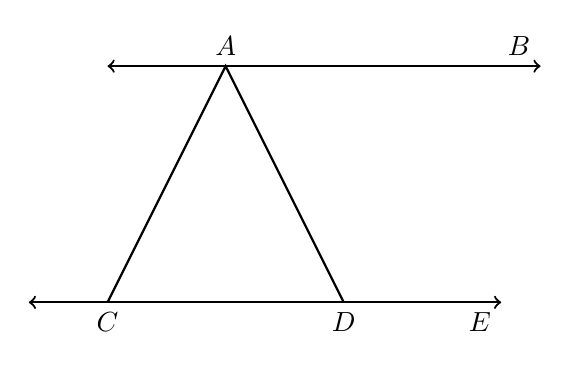
\begin{tikzpicture}
      \draw [<->, thick] (1,3)--(6.5,3) node[above left]{$B$};
      \draw [<->, thick] (0,0)--
        (5,0)--
        (6,0) node[below left]{$E$};
      \draw [-, thick] (1,0) node[below]{$C$}--
        (2.5,3) node[above]{$A$}--
        (4,0) node[below]{$D$};
    \end{tikzpicture}
    \end{flushright} \vspace{1.5cm}

\newpage

  \item Find the image of $P(3,1)$ after the translation $(x,y) \rightarrow (x-7,y+2)$. \hfill (1 star) \vspace{2cm}

  \item Translate $\triangle ABC$ by $(x,y) \rightarrow (x+5, y-2)$. Make a table of the coordinates and plot and label the image on the axes. \hfill (2 stars)
  \begin{flushright}
    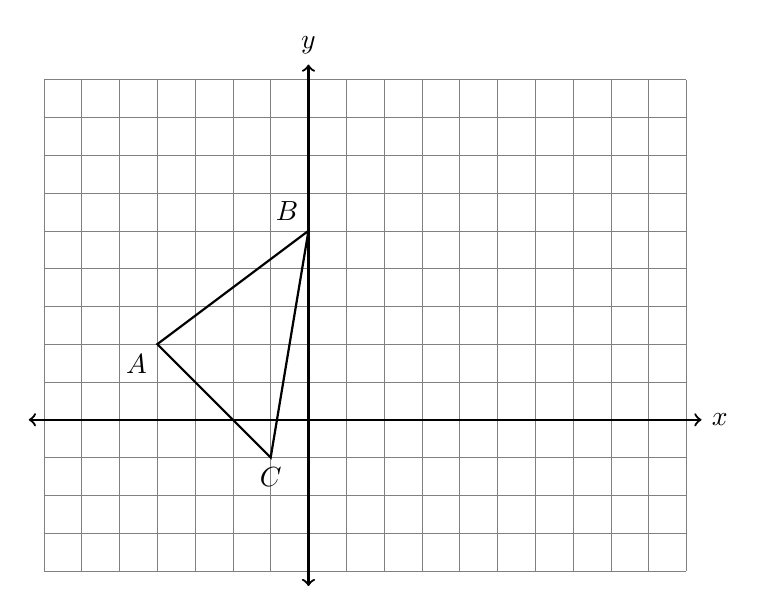
\begin{tikzpicture}[scale=.48]
      \draw [help lines] (-7,-4) grid (10,9);
      \draw [thick, <->] (-7.4,0) -- (10.4,0) node [right] {$x$};
      \draw [thick, <->] (0,-4.4)--(0,9.4) node [above] {$y$};  
      \draw [thick]
        (-4,2) node[below left] {$A$}--
        (0,5) node[above left] {$B$}--
        (-1,-1) node[below] {$C$}--cycle;  
  \end{tikzpicture}
  \end{flushright}

  \item A transformation maps $\triangle ABC \rightarrow \triangle A'B'C'$. Make a table of the coordinates of both triangles and fully specify the transformation. \hfill (3 stars)
  \begin{flushright}
    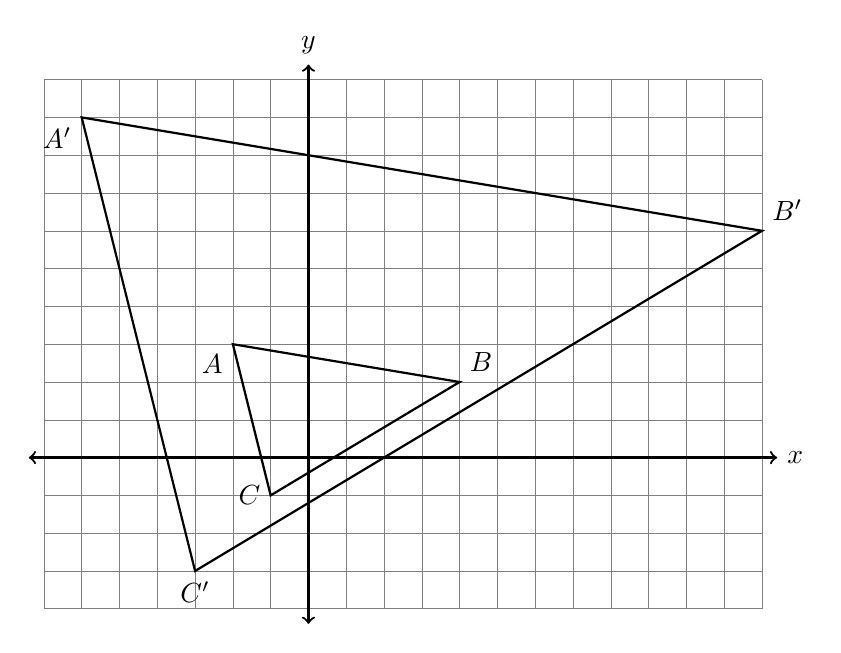
\begin{tikzpicture}[scale=.48]
      \draw [help lines] (-7,-4) grid (12,10);
      \draw [thick, <->] (-7.4,0) -- (12.4,0) node [right] {$x$};
      \draw [thick, <->] (0,-4.4)--(0,10.4) node [above] {$y$};  
      \draw [thick]
        (-2,3) node[below left] {$A$}--
        (4,2) node[above right] {$B$}--
        (-1,-1) node[left] {$C$}--cycle;
      \draw [thick]
        (-6,9) node[below left] {$A'$}--
        (12,6) node[above right] {$B'$}--
        (-3,-3) node[below] {$C'$}--cycle; 
  \end{tikzpicture}
  \end{flushright}

\newpage

  \item Two transformations are applied to $\triangle ABC$, first a dilation with scale factor $k=2$ centered at the origin, then a translation down 5 and to the right 3. Make a table of the coordinates showing $\triangle ABC \rightarrow \triangle A'B'C' \rightarrow \triangle A''B''C''$ and plot and label the images on the axes. \hfill (3 stars)
  \begin{flushright}
      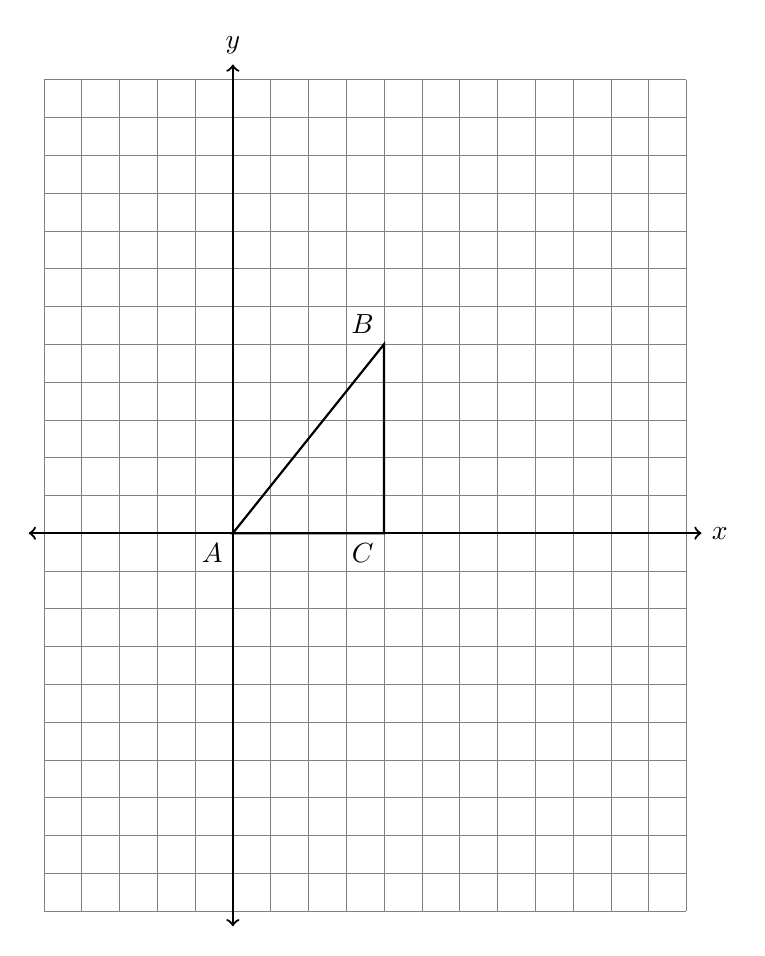
\begin{tikzpicture}[scale=.48]
      \draw [help lines] (-5,-10) grid (12,12);
      \draw [thick, <->] (-5.4,0) -- (12.4,0) node [right] {$x$};
      \draw [thick, <->] (0,-10.4)--(0,12.4) node [above] {$y$};  
      \draw [thick]
        (0,0) node[below left] {$A$}--
        (4,5) node[above left] {$B$}--
        (4,0) node[below left] {$C$}--cycle;  
    \end{tikzpicture}
  \end{flushright}
    

\end{enumerate}
\end{document}
